% Created 2020-08-29 Sat 18:59
% Intended LaTeX compiler: pdflatex
\documentclass[11pt]{article}
\usepackage[utf8]{inputenc}
\usepackage[T1]{fontenc}
\usepackage{graphicx}
\usepackage{grffile}
\usepackage{longtable}
\usepackage{wrapfig}
\usepackage{rotating}
\usepackage[normalem]{ulem}
\usepackage{amsmath}
\usepackage{textcomp}
\usepackage{amssymb}
\usepackage{capt-of}
\usepackage{hyperref}
\usepackage{listings}
\IfFileExists{./resources/style.sty}{\usepackage{./resources/style}}{}
\IfFileExists{./resources/referencing.sty}{\usepackage{./resources/referencing}}{}
\addbibresource{../Resources/references.bib}
\author{Ryan Greenup \& James Guerra}
\date{\today}
\title{The Emergence of Patterns in Nature and Chaos Theory}
\hypersetup{
 pdfauthor={Ryan Greenup \& James Guerra},
 pdftitle={The Emergence of Patterns in Nature and Chaos Theory},
 pdfkeywords={},
 pdfsubject={},
 pdfcreator={Emacs 27.1 (Org mode 9.4)}, 
 pdflang={English}}
\begin{document}

\maketitle
\tableofcontents


\section{Introduction\hfill{}\textsc{Ryan}}
\label{sec:org12b1af6}
This project, at the outset, was very broadly concerned with the use of \emph{Python} for
computer algebra. Much to the the reluctance of our supervisor we have however
resolved to look at a broad variety of tools (see section \ref{other-tools}),
in particular a language we wanted an opportunity to explore was \emph{Julia}
\cite{bezansonJuliaFreshApproach2017} \footnote{See section}.

In order to give the project a more focused direction we have decided to look into: \footnote{The amount of independence that our supervisor afforded us to
investigate other languages is something that we are both extremely grateful for.}

\begin{itemize}
\item The Emergence of patterns in Nature
\item Chaos Theory \& Dynamical Systems
\item Fractals
\end{itemize}

These three topics are very tightly connected and so it is difficult to look at
any one in a vacuum, they also almost necessitate the use of software packages
due to the fact that these phenomena appear to occur in recursive systems, more
over such software needs to perform very well under recursion and iteration
(making this a very good focus for this topic generally, and an excuse to work
with Julia as well).

\section{Programming Recursion\hfill{}\textsc{Ryan}}
\label{sec:org0c349fe}
As an introduction to \emph{Python} generally, we undertook many problem questions which have been omitted from this outline, however, this one in particular offered an interesting insight into the difficulties we may encounter when dealing with recursive systems.
\subsection{Iteration and Recursion}
\label{series-and-recursion}
Consider the series shown in \eqref{eq:rec-ser}\footnote{This problem is taken from Project A (44) of Dr. Hazrat's \emph{Mathematica: A Problem Centred Approach} \cite{hazratMathematicaProblemCenteredApproach2015}} :

\begin{align}
    g\left( k \right) &=  \frac{\sqrt{2} }{2} \cdot   \frac{\sqrt{2+  \sqrt{3}}  }{3} \frac{\sqrt{2 +  \sqrt{3 +  \sqrt{4} } } }{4} \cdot  \ldots \frac{\sqrt{2 +  \sqrt{3 +  \ldots +  \sqrt{k} } } }{k} \label{eq:rec-ser}
\end{align}

let's modify this for the sake of discussion:

\begin{align}
h\left( k \right) = \frac{\sqrt{2}  }{2} \cdot  \frac{\sqrt{3 +  \sqrt{2} } }{3} \cdot  \frac{\sqrt{4 +  \sqrt{3 +  \sqrt{2} } } }{4} \cdot  \ldots \cdot  \frac{\sqrt{k +  \sqrt{k - 1 +  \ldots \sqrt{3 + \sqrt{2}  } } } }{k} \label{eq:rec-ser-mod}
\end{align}

The function \(h\) can be expressed by the series:

$$\begin{aligned}
h\left( k \right) = \prod^k_{i = 2} \left( \frac{f_i}{i}  \right)  \quad : \quad f_i = \sqrt{i +  f_{i - 1}}, \enspace f_{1} = 1
\end{aligned}$$

Within \emph{Python}, it isn't difficult to express \(h\), the series can be expressed
with recursion as shown in listing \ref{rec-one}, this is a very natural way to define
series and sequences and is consistent with familiar mathematical thought and
notation. Individuals more familiar with programming than analysis may find it
more comfortable to use an iterator as shown in listing \ref{it-one}.

\lstset{language=Python,label=rec-one,caption={Solving \eqref{eq:rec-ser-mod} using recursion.},captionpos=b,numbers=none}
\begin{lstlisting}
from sympy import *
def h(k):
    if k > 2:
        return f(k) * f(k-1)
    else:
        return 1

def f(i):
    expr = 0
    if i > 2:
        return sqrt(i + f(i -1))
    else:
        return 1
\end{lstlisting}


\lstset{language=Python,label=it-one,caption={Solving \eqref{eq:rec-ser-mod} by using a \texttt{for} loop.},captionpos=b,numbers=none}
\begin{lstlisting}
  from sympy import *
  def h(k):
      k = k + 1 # OBOB
      l = [f(i) for i in range(1,k)]
      return prod(l)

  def f(k):
      expr = 0
      for i in range(2, k+2):
          expr = sqrt(i + expr, evaluate=False)
      return expr/(k+1)
\end{lstlisting}

Any function that can be defined by using iteration, can always be defined via
recursion and vice versa
\cite{bohmReducingRecursionIteration1988,bohmReducingRecursionIteration1986}
(see also
\cite{smolarskiMath60Notes2000,IterationVsRecursion2016} ),

there is however, evidence to suggest that recursive functions are easier for
people to understand \cite{benanderEmpiricalAnalysisDebugging2000} and so should
be favoured. Although independent research has shown that the specific language
chosen can have a bigger effect on how well recursive as opposed to iterative
code is understood \cite{sinhaCognitiveFitEmpirical1992}.

The relevant question is ``\emph{which method is often more appropriate}?'', generally
the process for determining which is more appropriate is to the effect of:

\begin{enumerate}
\item Write the problem in a way that is easier to write or is more
appropriate for demonstration
\item If performance is a concern then consider restructuring in favour of iteration
\begin{itemize}
\item For interpreted languages such \textbf{\emph{R}} and \emph{Python}, loops are usually
faster, because of the overheads involved in creating functions
\cite{smolarskiMath60Notes2000} although there may be exceptions to this and
I'm not sure if this would be true for compiled languages such as \emph{Julia},
\emph{Java}, \textbf{\emph{C}} etc.
\end{itemize}
\end{enumerate}

\subsubsection{Some Functions are more difficult to express with Recursion in}
\label{some-functions-are-more-difficult-to-express-with-recursion-in-python}
Attacking a problem recursively isn't always the best approach however. Consider the function \(g\left( k \right)\) from \eqref{eq:rec-ser}:


\begin{align}
    g\left( k \right) &=  \frac{\sqrt{2} }{2} \cdot   \frac{\sqrt{2+  \sqrt{3}}  }{3} \frac{\sqrt{2 +  \sqrt{3 +  \sqrt{4} } } }{4} \cdot  \ldots \frac{\sqrt{2 +  \sqrt{3 +  \ldots +  \sqrt{k} } } }{k} \nonumber \\
    &=  \prod^k_{i = 2} \left( \frac{f_i}{i}  \right) \quad : \quad f_{i} = \sqrt{i +  f_{i+1}} \nonumber
\end{align}

Observe that the difference between \eqref{eq:rec-ser} and \eqref{eq:rec-ser-mod} is
that the sequence essentially \emph{looks} forward, not back. To solve using a \texttt{for}
loop, this distinction is a non-concern because the list can be reversed using a built-in
such as \texttt{rev}, \texttt{reversed} or \texttt{reverse} in \emph{Python}, \textbf{\emph{R}} and \emph{Julia}
respectively, which means the same expression can be implemented.

To implement with recursion however, the series needs to be restructured and
this can become a little clumsy, see \eqref{eq:clumsy}:

\begin{align}
    g\left( k \right) &=  \prod^k_{i = 2} \left( \frac{f_i}{i}  \right) \quad : \quad f_{i} = \sqrt{\left( k- i \right)  +  f_{k - i - 1}} \label{eq:clumsy}
\end{align}

Now the function could be performed recursively in \emph{Python} in a similar way as
shown in listing \ref{rec-two}, but it's also significantly more confusing because the
\(f\) function now has \(k\) as a parameter and this is only made significantly more
complicated by the differing implementations of variable scope across common
languages used in Mathematics and Data science such as \texttt{bash}, \textbf{\emph{R}}, \emph{Julia}, \emph{Python}.

If however, the \texttt{for} loop approach was implemented, as shown in listing
\ref{iter-two}, the function would not significantly change, because the \texttt{reversed()} function can be
used to flip the list around.

What this demonstrates is that taking a different approach to simply describing
this function can lead to big differences in the complexity involved in solving
this problem.

\lstset{language=Python,label=rec-two,caption={Using Recursion to Solve \eqref{eq:rec-ser}},captionpos=b,numbers=none}
\begin{lstlisting}
from sympy import *
def h(k):
    if k > 2:
        return f(k, k) * f(k, k-1)
    else:
        return 1

def f(k, i):
    if k > i:
        return 1
    if i > 2:
        return sqrt((k-i) + f(k, k - i -1))
    else:
        return 1
\end{lstlisting}


\lstset{language=Python,label=iter-two,caption={Using Iteration to Solve \eqref{eq:rec-ser}},captionpos=b,numbers=none}
\begin{lstlisting}
from sympy import *
def h(k):
    k = k + 1 # OBOB
    l = [f(i) for i in range(1,k)]
    return prod(l)

def f(k):
    expr = 0
    for i in reversed(range(2, k+2)):
        expr = sqrt(i + expr, evaluate=False)
    return expr/(k+1)
\end{lstlisting}

\section{Fibonacci Sequence\hfill{}\textsc{Ryan:James}}
\label{sec:org5f7a35f}
\subsection{Introduction\hfill{}\textsc{Ryan}}
\label{sec:org5df751a}
The \emph{Fibonacci Sequence} and \emph{Golden Ratio} share a deep connection\footnote{See section} and occur in patterns observed in nature very frequently
(see
\cite{shellyallenFibonacciNature,benedettapalazzoNumbersNatureFibonacci2016,MinarovaNikoletta2014TFSN,NatureGoldenRatio2018,robertlambHowAreFibonacci2008,ronknottFibonacciNumbersGolden2016}), an example of such an occurence is discussed in section \ref{sunflower-example}.


In this section we lay out a strategy to find an analytic solution to the
\emph{Fibonacci Sequence} by relating it to a continuous series and generalise this
approach to any homogenous linear recurrence relation.

This details some open mathematical work for the project and our hope is that by
identifying relationships between discrete and continuous systems generall we
will be able to draw insights with regard to the occurrence of patterns related
to the \emph{Fibonacci Sequence} and \emph{Golden Ratio} in nature.

\subsection{Computational Approach\hfill{}\textsc{Ryan}}
\label{define-the-fibonacci-numbers}
Given that much of our work will involve computational analysis and simulation we begin with a strategy to solve the sequence computationally.

The \emph{Fibonacci} Numbers are given by:

\begin{align}
F_n = F_{n-1} + F_{n-2} \label{eq:fib-def}
\end{align}

This type of recursive relation can be expressed in \emph{Python} by using recursion,
as shown in listing \ref{fib-rec-0}, however using this function will reveal that it
is extraordinarily slow, as shown in listing \ref{time-slow}, this is because the
results of the function are not cached and every time the function is called
every value is recalculated\footnote{Dr. Hazrat mentions something similar in his book with respect to
\emph{Mathematica}\textsuperscript{\textregistered}
\cite[Ch. 13]{hazratMathematicaProblemCenteredApproach2015}}, meaning that the workload scales in
exponential as opposed to polynomial time.

The \texttt{functools} library for python includes the \texttt{@functools.lru\_cache} decorator
which will modify a defined function to cache results in memory
\cite{FunctoolsHigherorderFunctions}, this means that the recursive function will
only need to calculate each result once and it will hence scale in polynomial
time, this is implemented in listing \ref{fib-cache}.


\lstset{language=Python,label=fib-rec-0,caption={Defining the \emph{Fibonacci Sequence} \eqref{eq:fib-def} using Recursion},captionpos=b,numbers=none}
\begin{lstlisting}
  def rec_fib(k):
      if type(k) is not int:
          print("Error: Require integer values")
          return 0
      elif k == 0:
          return 0
      elif k <= 2:
          return 1
      return rec_fib(k-1) + rec_fib(k-2)
\end{lstlisting}

\lstset{language=Python,label=time-slow,caption={Using the function from listing \ref{fib-rec-0} is quite slow.},captionpos=b,numbers=none}
\begin{lstlisting}
  start = time.time()
  rec_fib(35)
  print(str(round(time.time() - start, 3)) + "seconds")

## 2.245seconds
\end{lstlisting}


\lstset{language=Python,label=fib-cache,caption={Caching the results of the function previously defined \ref{time-slow}},captionpos=b,numbers=none}
\begin{lstlisting}
  from functools import lru_cache

  @lru_cache(maxsize=9999)
  def rec_fib(k):
      if type(k) is not int:
          print("Error: Require Integer Values")
          return 0
      elif k == 0:
          return 0
      elif k <= 2:
          return 1
      return rec_fib(k-1) + rec_fib(k-2)


start = time.time()
rec_fib(35)
print(str(round(time.time() - start, 3)) + "seconds")
## 0.0seconds
\end{lstlisting}

\lstset{language=Python,label= ,caption= ,captionpos=b,numbers=none}
\begin{lstlisting}
  start = time.time()
  rec_fib(6000)
  print(str(round(time.time() - start, 9)) + "seconds")

## 8.3923e-05seconds
\end{lstlisting}

Restructuring the problem to use iteration will allow for even greater performance as demonstrated by finding \(F_{10^{6}}\) in listing \ref{fib-iter}. Using a compiled language such as \emph{Julia} however would be thousands of times faster still, as demonstrated in listing \ref{julia-fib}.



\lstset{language=Python,label=fib-iter,caption={Using Iteration to Solve the Fibonacci Sequence},captionpos=b,numbers=none}
\begin{lstlisting}
  def my_it_fib(k):
      if k == 0:
          return k
      elif type(k) is not int:
          print("ERROR: Integer Required")
          return 0
      # Hence k must be a positive integer

      i  = 1
      n1 = 1
      n2 = 1

      # if k <=2:
      #     return 1

      while i < k:
         no = n1
         n1 = n2
         n2 = no + n2
         i = i + 1
      return (n1)

  start = time.time()
  my_it_fib(10**6)
  print(str(round(time.time() - start, 9)) + "seconds")

 ## 6.975890398seconds
\end{lstlisting}

\lstset{language=julia,label=julia-fib,caption={Using Julia with an iterative approach to solve the 1 millionth fibonacci number},captionpos=b,numbers=none}
\begin{lstlisting}
function my_it_fib(k)
    if k == 0
        return k
    elseif typeof(k) != Int
        print("ERROR: Integer Required")
        return 0
    end
    # Hence k must be a positive integer

    i  = 1
    n1 = 1
    n2 = 1

    # if k <=2:
    #     return 1
    while i < k
       no = n1
       n1 = n2
       n2 = no + n2
       i = i + 1
    end
    return (n1)
end

@time my_it_fib(10^6)

##  my_it_fib (generic function with 1 method)
##    0.000450 seconds
\end{lstlisting}

In this case however an analytic solution can be found by relating discrete
mathematical problems to continuous ones as discussed below at section .
\subsection{Exponential Generating Functions}
\label{exp-gen-func-fib-seq}
\subsubsection{Motivation\hfill{}\textsc{Ryan}}
\label{motivation}
Consider the \emph{Fibonacci Sequence} from \eqref{eq:fib-def}:


\begin{align}
    a_{n}&= a_{n - 1} + a_{n - 2} \nonumber \\
\iff a_{n+  2} &= a_{n+  1} +  a_n \label{eq:fib-def-shift}
\end{align}


from observation, this appears similar in structure to the following \emph{ordinary
differential equation}, which would be fairly easy to deal with:


\begin{align*}
f''\left( x \right)- f'\left( x \right)- f\left( x \right)=  0
\end{align*}

By ODE Theory we have \(y \propto e^{m_{i}x}, \enspace i = 1, 2\):

\begin{align*}
f\left( x \right)= e^{mx} = \sum^{\infty}_{n= 0}   \left[ r^{m} \frac{x^n}{n!} \right]
\end{align*}

So using some sort of a transformation involving a power series may help to
relate the discrete problem back to a continuous one.

\subsubsection{Example\hfill{}\textsc{Ryan}}
\label{solving-the-sequence}
Consider using the following generating function, (the derivative of the
generating function as in \eqref{eq:exp-gen-def-2} and \eqref{eq:exp-gen-def-3} is
provided in section \ref{Derivative-exp-gen-function})




\begin{align}
    f\left( x \right) &=  \sum^{\infty}_{n= 0}   \left[ a_{n} \cdot  \frac{x^n}{n!} \right]   \label{eq:exp-gen-def-1} \\
 \implies   f'\left( x \right) &=  \sum^{\infty}_{n= 0}   \left[ a_{n+1} \cdot  \frac{x^n}{n!} \right]   \label{eq:exp-gen-def-2} \\
\implies    f''\left( x \right) &=  \sum^{\infty}_{n= 0}   \left[ a_{n+2} \cdot  \frac{x^n}{n!} \right]   \label{eq:exp-gen-def-3}
\end{align}


So the recursive relation from \eqref{eq:fib-def-shift}  could be expressed :


\begin{align*}
a_{n+  2}    &= a_{n+  1} +  a_{n}\\
\frac{x^n}{n!}   a_{n+  2}    &= \frac{x^n}{n!}\left( a_{n+  1} +  a_{n}  \right)\\
\sum^{\infty}_{n= 0} \left[ \frac{x^n}{n!}   a_{n+  2} \right]        &= \sum^{\infty}_{n= 0}   \left[ \frac{x^n}{n!} a_{n+  1} \right]  + \sum^{\infty}_{n= 0}   \left[ \frac{x^n}{n!} a_{n}  \right]  \\
\end{align*}

And hence by applying \eqref{eq:exp-gen-def-1}:

\begin{align}
f''\left( x \right) &= f'\left( x \right)+  f\left( x \right)
\end{align}


Using the theory of higher order linear differential equations with
constant coefficients it can be shown:


\begin{align*}
f\left( x \right)= c_1 \cdot  \mathrm{exp}\left[ \left( \frac{1- \sqrt{5} }{2} \right)x \right] +  c_2 \cdot  \mathrm{exp}\left[ \left( \frac{1 +  \sqrt{5} }{2} \right) \right]
\end{align*}


By equating this to the power series:


\begin{align*}
f\left( x \right)&= \sum^{\infty}_{n= 0}   \left[ \left( c_1\left( \frac{1- \sqrt{5} }{2} \right)^n +  c_2 \cdot  \left( \frac{1+ \sqrt{5} }{2} \right)^n \right) \cdot  \frac{x^n}{n} \right]
\end{align*}


Now given that:


\begin{align*}
f\left( x \right)= \sum^{\infty}_{n= 0}   \left[ a_n \frac{x^n}{n!} \right]
\end{align*}


We can conclude that:


\begin{align*}
a_n = c_1\cdot  \left( \frac{1- \sqrt{5} }{2} \right)^n +  c_2 \cdot  \left( \frac{1+  \sqrt{5} }{2} \right)
\end{align*}


By applying the initial conditions:


\begin{align*}
a_0= c_1 +  c_2  \implies  c_1= - c_2\\
a_1= c_1 \left( \frac{1+ \sqrt{5} }{2} \right) -  c_1 \frac{1-\sqrt{5} }{2}  \implies  c_1 = \frac{1}{\sqrt{5} }
\end{align*}


And so finally we have the solution to the \emph{Fibonacci Sequence} \ref{eq:fib-def-shift}:


\begin{align}
    a_n &= \frac{1}{\sqrt{5} } \left[ \left( \frac{1+  \sqrt{5} }{2}  \right)^n -  \left( \frac{1- \sqrt{5} }{2} \right)^n \right] \nonumber \\
&= \frac{\varphi^n - \psi^n}{\sqrt{5} } \nonumber\\
&=\frac{\varphi^n -  \psi^n}{\varphi - \psi} \label{eq:fib-sol}
\end{align}


where:

\begin{itemize}
\item \(\varphi = \frac{1+ \sqrt{5} }{2} \approx 1.61\ldots\)
\item \(\psi = 1-\varphi = \frac{1- \sqrt{5} }{2} \approx 0.61\ldots\)
\end{itemize}

\subsubsection{Derivative of the Exponential Generating Function}
\label{Derivative-exp-gen-function}
\paragraph{Base\hfill{}\textsc{Ryan}}
\label{sec:org05e2ee4}
Differentiating the exponential generating function has the effect of shifting the sequence to the backward: \cite{lehmanReadingsMathematicsComputer2010}

\begin{align}
    f\left( x \right) &= \sum^{\infty}_{n= 0}   \left[ a_n \frac{x^n}{n!} \right] \label{eq:exp-pow-series} \\
f'\left( x \right)) &= \frac{\mathrm{d} }{\mathrm{d} x}\left( \sum^{\infty}_{n= 0}   \left[ a_n \frac{x^n}{n!} \right]  \right) \nonumber \\
&= \frac{\mathrm{d}}{\mathrm{d} x} \left( a_0 \frac{x^0}{0!} +  a_1 \frac{x^1}{1!} +  a_2 \frac{x^2}{2!}+  a_3 \frac{x^3}{3! } +  \ldots \frac{x^k}{k!} \right) \nonumber \\
&= \sum^{\infty}_{n= 0}   \left[ \frac{\mathrm{d} }{\mathrm{d} x}\left( a_n \frac{x^n}{n!} \right) \right] \nonumber \\
&= \sum^{\infty}_{n= 0}   {\left[{ \frac{a_n}{{\left({ n- 1 }\right)!}} } x^{n- 1}  \right]} \nonumber \\
\implies f'(x) &= \sum^{\infty}_{n= 0}   {\left[{ \frac{x^n}{n!}a_{n+  1} }\right]} \label{eq:exp-pow-series-sol}
\end{align}

\paragraph{Bridge\hfill{}\textsc{James}}
\label{sec:org5bf926e}
This can be shown for all derivatives by way of induction, for

\begin{align}
f^{(k)}\left(x\right) = \sum_{n=0}^\infty\frac{a_{n+k}\cdot x^n}{n!} \quad \text{for}~k \ge 0
\end{align}

Assume that. \(f^{(k)}\left(x\right) = \sum_{n=0}^\infty\frac{a_{n+k}\cdot x^n}{n!}\)

Using this assumption, prove for the next element \(k+1\)

We need \(f^{(k+1)}(x) = \sum_{n=0}^\infty\frac{a_{n+k+1}\cdot x^n}{n!}\)

\begin{align*}
    \text{LHS} &= f^{(k+1)}(x)\\
    &= \frac{\mathrm{d}}{\mathrm{d}x}\left(f^{(k)}(x)\right)\\
    &= \frac{\mathrm{d}}{\mathrm{d}x}\left(\sum_{n=0}^\infty\frac{a_{n+k}\cdot x^n}{n!}\right)\quad \text{by assumption}\\
    &= \sum_{n=0}^\infty\frac{a_{n+k}\cdot n\cdot x^{n-1}}{n!}\\
    &= \sum_{n=1}^\infty\frac{a_{n+k}\cdot x^{n-1}}{(n-1)!}\\
    &= \sum_{n=0}^\infty\frac{a_{n+k+1}\cdot x^{n}}{n!}\\
    &= \text{RHS}
\end{align*}

Thus, if the derivative of the series shown in \eqref{eq:exp-gen-def-1} shifts the
sequence across, then every derivative thereafter does so as well, because the
first derivative has been shown to express this property
\eqref{eq:exp-pow-series-sol}, all derivates will.

\subsubsection{Homogeneous Proof\hfill{}\textsc{Ryan:James}}
\label{sec:org23dbad4}
An equation of the form:

\begin{align}
\sum^{n}_{i=0} \left[ c_{i} \cdot f^{(i)}(x) \right] = 0 \label{eq:hom-ode}
\end{align}

is said to be a homogenous linear ODE: \cite[Ch. 2]{zillDifferentialEquations2009a}

\begin{description}
\item[{Linear}] because the equation is linear with respect to \(f(x)\)
\item[{Ordinary}] because there are no partial derivatives (e.g. \(\frac{\partial }{\partial x}{\left({ f{\left({ x }\right)} }\right)}\)  )
\item[{Differential}] because the derivates of the function are concerned
\item[{Homogenous}] because the \textbf{\emph{RHS}} is 0
\begin{itemize}
\item A non-homogeous equation would have a non-zero RHS
\end{itemize}
\end{description}

There will be \(k\) solutions to a \(k^{\mathrm{th}}\) order linear ODE, each may be summed to produce a superposition which will also be a solution to the equation, \cite[Ch. 4]{zillDifferentialEquations2009a}  this will be considered as the desired complete solution (and this will be shown to be the only solution for the recurrence relation \eqref{eq:recurrence-relation-def}). These \(k\) solutions will be in one of two forms:

\begin{enumerate}
\item \(f(x)=c_{i} \cdot e^{m_{i}x}\)
\item \(f(x)=c_{i} \cdot x^{j}\cdot e^{m_{i}x}\)
\end{enumerate}

where:

\begin{itemize}
\item \(\sum^{k}_{i=0}\left[  c_{i}m^{k-i} \right] = 0\)
\begin{itemize}
\item This is referred to the characteristic equation of the recurrence relation or ODE \cite{levinSolvingRecurrenceRelations2018}
\end{itemize}
\item \(\exists i,j \in \mathbb{Z}^{+} \cap \left[0,k\right]\)
\begin{itemize}
\item These is often referred to as repeated roots \cite{levinSolvingRecurrenceRelations2018,zillMatrixExponential2009} with a multiplicity corresponding to the number of repetitions of that root \cite[\textsection 3.2]{nicodemiIntroductionAbstractAlgebra2007}
\end{itemize}
\end{itemize}

\paragraph{Unique Roots of Characteristic Equation\hfill{}\textsc{Ryan}}
\label{uniq-roots-recurrence}
\subparagraph{Example}
\label{sec:org36d0597}
An example of a recurrence relation with all unique roots is the fibonacci sequence, as described in section \ref{solving-the-sequence}.
\subparagraph{Proof}
\label{sec:orgc3b462c}
Consider the linear recurrence relation \eqref{eq:recurrence-relation-def}:

\begin{align}
\sum^{n}_{i= 0}   \left[ c_i \cdot  a_i \right] = 0, \quad \exists c \in
\mathbb{R}, \enspace \forall i<k\in\mathbb{Z}^+ \nonumber \label{eq:recurrence-relation-def}
\end{align}
This implies:


\begin{align}
    \sum^{\infty}_{n= 0}   \left[ \sum^{k}_{i= 0}   \left[ \frac{x^n}{n!} c_i a_n \right]  \right]  &= 0 \\
    \sum^{\infty}_{n= 0}    \sum^{k}_{i= 0}    \frac{x^n}{n!} c_i a_n    &= 0 \\
        \sum^{k}_{i= 0} c_i \sum^{\infty}_{n= 0}    \frac{x^n}{n!}  a_n    &= 0
\end{align}

By implementing the exponential generating function as shown in
\eqref{eq:exp-gen-def-1}, this provides:

\begin{align}
   \sum^{k}_{i= 0}   \left[ c_i f^{\left( i \right)}\left( x \right) \right]
\end{align}


Now assume that the solution exists and all roots of the characteristic polynomial are unique (i.e. the solution is of the form \(f{\left({ x }\right)} \propto e^{m_i x}: \quad m_i \neq m_j \forall i\neq j\)), this implies that  \cite[Ch. 4]{zillDifferentialEquations2009a} :

\begin{align}
    f{\left({ x }\right)} = \sum^{k}_{i= 0}   {\left[{ k_i e^{m_i x} }\right]}, \quad \exists m,k \in \mathbb{C} \nonumber
\end{align}

This can be re-expressed in terms of the exponential power series, in order to relate the solution of the function \(f{\left({ x }\right)}\) back to a solution of the sequence \(a_n\), (see section for a derivation of the exponential power series):

\begin{align}
    \sum^{k}_{i= 0}   {\left[{ k_i e^{m_i x}  }\right]}  &= \sum^{k}_{i= 0}   {\left[{ k_i \sum^{\infty}_{n= 0}   \frac{{\left({ m_i x }\right)}^n}{n!}  }\right]}  \nonumber \\
							 &= \sum^{k}_{i= 0}  \sum^{\infty}_{n= 0}   k_i m_i^n \frac{x^n}{n!} \nonumber\\
							 &=    \sum^{\infty}_{n= 0} \sum^{k}_{i= 0}   k_i m_i^n \frac{x^n}{n!} \nonumber \\
							 &= \sum^{\infty}_{n= 0} {\left[{ \frac{x^n}{n!}  \sum^{k}_{i=0}   {\left[{ k_im^n_i }\right]}  }\right]}, \quad \exists k_i \in \mathbb{C}, \enspace \forall i \in \mathbb{Z}^+\cap {\left[{ 1, k }\right]}     \label{eq:unique-root-sol-power-series-form}
\end{align}


Recall the definition of the generating function from \eqref{eq:exp-gen-def-1}, by relating this to \eqref{eq:unique-root-sol-power-series-form}:

\begin{align}
    f{\left({ x }\right)} &= \sum^{\infty}_{n= 0}   {\left[{  \frac{x^n}{n!} a_n }\right]} \nonumber \\
&= \sum^{\infty}_{n= 0} {\left[{ \frac{x^n}{n!}  \sum^{k}_{i=0}   {\left[{ k_im^n_i }\right]}  }\right]}  \nonumber \\
      \implies  a_n &= \sum^{k}_{n= 0} {\left[{ k_im_i^n }\right]}     \nonumber \\ \nonumber
\square
\end{align}

This can be verified by the fibonacci sequence as shown in section \ref{solving-the-sequence}, the solution to the characteristic equation is \(m_1 = \varphi, m_2 = {\left({ 1-\varphi }\right)}\) and the corresponding solution to the linear ODE and recursive relation are:

\begin{alignat}{4}
    f{\left({ x }\right)} &= &c_1 e^{\varphi x} +  &c_2 e^{{\left({ 1-\varphi }\right)} x}, \quad &\exists c_1, c_2 \in \mathbb{R} \subset \mathbb{C} \nonumber \\
    \iff  a_n &= &k_1 n^{\varphi} +  &k_2 n^{1- \varphi}, &\exists k_1, k_2 \in \mathbb{R} \subset \mathbb{C} \nonumber
\end{alignat}

\paragraph{Repeated Roots of Characteristic Equation\hfill{}\textsc{Ryan}}
\label{rep-roots-recurrence}
\subparagraph{Example}
\label{sec:org3fea767}
Consider the following recurrence relation:

\begin{align}
    a_n -  10a_{n+ 1} +  25a_{n+  2}&= 0 \label{eq:hom-repeated-roots-recurrence} \\
    \implies  \sum^{\infty}_{n= 0}   {\left[{ a_n \frac{x^n}{n!} }\right]} - 10 \sum^{\infty}_{n= 0}   {\left[{ \frac{x^n}{n!}+    }\right]} + 25 \sum^{\infty}_{n= 0 }   {\left[{  a_{n+  2 }\frac{x^n}{n!} }\right]}&= 0 \nonumber
\end{align}

By applying the definition of the exponential generating function at \eqref{eq:exp-gen-def-1} :

\begin{align}
    f''{\left({ x }\right)}- 10f'{\left({ x }\right)}+  25f{\left({ x }\right)}= 0 \nonumber \label{eq:rep-roots-func-ode}
\end{align}

By implementing the already well-established theory of linear ODE's, the
characteristic equation for \eqref{eq:rep-roots-func-ode} can be expressed as:

\begin{align}
    m^2- 10m+  25 = 0 \nonumber \\
    {\left({ m- 5 }\right)}^2 = 0 \nonumber \\
    m= 5 \label{eq:rep-roots-recurrence-char-sol}
\end{align}

Herein lies a complexity, in order to solve this, the solution produced from \eqref{eq:rep-roots-recurrence-char-sol} can be used with the \emph{Reduction of Order} technique to produce a solution that will be of the form \cite[\textsection 4.3]{zillMatrixExponential2009}.

\begin{align}
    f{\left({ x }\right)}= c_1e^{5x} +  c_2 x e^{5x} \label{eq:rep-roots-ode-sol}
\end{align}

\eqref{eq:rep-roots-ode-sol} can be expressed in terms of the exponential power series in order to try and relate the solution for the function back to the generating function,
observe however the following power series identity (TODO Prove this in section ):

\begin{align}
    x^ke^x &= \sum^{\infty}_{n= 0}   {\left[{ \frac{x^n}{{\left({ n- k }\right)}!} }\right]}, \quad \exists k \in \mathbb{Z}^+ \label{eq:uniq-roots-pow-series-ident}
\end{align}

by applying identity \eqref{eq:uniq-roots-pow-series-ident} to equation \eqref{eq:rep-roots-ode-sol}

\begin{align}
    \implies  f{\left({ x }\right)} &= \sum^{\infty}_{n= 0}   {\left[{ c_1 \frac{{\left({ 5x }\right)}^n}{n!} }\right]}  +  \sum^{\infty}_{n= 0}   {\left[{ c_2 n \frac{{\left({ 5x^n }\right)}}{n{\left({ n-1 }\right)}!} }\right]} \nonumber \\
 &= \sum^{\infty}_{n= 0}   {\left[{ \frac{x^n}{n!} {\left({ c_{1}5^n +  c_2 n 5^n   }\right)} }\right]} \nonumber
\end{align}

Given the defenition of the exponential generating function from \eqref{eq:exp-gen-def-1}

\begin{align}
    f{\left({ x }\right)}&=     \sum^{\infty}_{n= 0}   {\left[{ a_n \frac{x^n}{n!} }\right]} \nonumber \\
    \iff a_n &= c_{15}^n +  c_2n_5^n \nonumber \\ \nonumber
    \ \nonumber \\
    \square \nonumber
\end{align}
\subparagraph{Proof}
\label{sec:org15a352f}
In order to prove the the solution for a \(k^{\mathrm{th}}\) order recurrence relation with \(k\) repeated


Consider a recurrence relation of the form:

\begin{align}
     \sum^{k}_{n= 0}   {\left[{ c_i a_n }\right]}  = 0 \nonumber \\
      \implies  \sum^{\infty}_{n= 0}   \sum^{k}_{i= 0}   c_i a_n \frac{x^n}{n!} = 0 \nonumber \\
      \sum^{k}_{i= 0}   \sum^{\infty}_{n= 0}   c_i a_n \frac{x^n}{n!} \nonumber
\end{align}

By substituting for the value of the generating function (from \eqref{eq:exp-gen-def-1}):

\begin{align}
    \sum^{k}_{i= 0}   {\left[{ c_if^{{\left({ k }\right)}}  {\left({ x }\right)}    }\right]} \label{eq:gen-form-rep-roots-ode}
\end{align}

Assume that \eqref{eq:gen-form-rep-roots-ode} corresponds to a charecteristic polynomial with only 1 root of multiplicity \(k\), the solution would hence be of the form:

\begin{align}
			 & \sum^{k}_{i= 0}   {\left[{ c_i m^i }\right]} = 0 \wedge m=B, \enspace  \exists! B \in \mathbb{C} \nonumber \\
 \implies      f{\left({ x }\right)}&= \sum^{k}_{i= 0}   {\left[{ x^i A_i e^{mx} }\right]}, \quad \exists A \in \mathbb{C}^+, \enspace \forall i \in {\left[{ 1,k }\right]} \cap \mathbb{N}  \label{eq:sol-rep-roots-ode} \\
\end{align}

If we assume that (see section \ref{power-series-comb}):

\begin{align}
k \in \mathbb{Z} \implies x^k e^x = \sum^{\infty}_{n= 0} {\left[{ \frac{x^n}{{\left({ n- k }\right)}!} }\right]}     \label{eq:power-series-comb}
\end{align}

By applying this to \eqref{eq:sol-rep-roots-ode} :

\begin{align}
f{\left({ x }\right)}&=     \sum^{k}_{i= 0}   {\left[{ A_i \sum^{\infty}_{n= 0}   {\left[{ \frac{{\left({ x m }\right)}^n}{{\left({ n- i }\right)}!} }\right]}  }\right]} \nonumber \\
&=     \sum^{\infty}_{n= 0}   {\left[{ \sum^{k}_{i=0} {\left[{ \frac{x^n}{n!}  \frac{n!}{{\left({ n- i }\right)}} A_i m^n }\right]}       }\right]} # \\
&=     \sum^{\infty}_{n= 0} {\left[{ \frac{x^n}{n!}   \sum^{k}_{i=0} {\left[{  \frac{n!}{{\left({ n- i }\right)}} A_i m^n }\right]}       }\right]}
\end{align}

Recall the generating function that was used to get \ref{eq:gen-form-rep-roots-ode}:

\begin{align}
f{\left({ x }\right)}&= \sum^{\infty}_{n= 0}   {\left[{ a_n \frac{x^n}{n!} }\right]}      \nonumber \\
 \implies  a_n &= \sum^{k}_{i= 0}   {\left[{ A_i \frac{n!}{{\left({ n- i }\right)}!} m^n  }\right]} \nonumber \\
 &= \sum^{k}_{i= 0}   {\left[{ m^n A_i \prod_{0}^{k} {\left[{ n- {\left({ i- 1 }\right)} }\right]}   }\right]}
& \intertext{$\because \enspace i \leq k$} \notag \\
 &= \sum^{k}_{i= 0} {\left[{ A_i^* m^n n^i }\right]}, \quad \exists A_i \in \mathbb{C}, \enspace \forall i\leqk \in \mathbb{Z}^+ \nonumber \\
\ \nonumber \\
\square \nonumber
\end{align}

\paragraph{General Proof}
\label{general-gen-func-proof}
In sections \ref{uniq-roots-recurrence} and \ref{uniq-roots-recurrence}
it was shown that a recurrence relation can be related to an ODE and then that
solution can be transformed to provide a solution for the recurrence relation,
when the charecteristic polynomial has either complex roots or 1 repeated root.
Generally the solution to a linear ODE will be a superposition of solutions for
each root, repeated or unique and so a goal of our research will be to put this
together to find a general solution for homogenous linear recurrence relations.

Sketching out an approach for this:

\begin{itemize}
\item Use the Generating function to get an ODE
\item The ODE will have a solution that is a combination of the above two forms
\item The solution will translate back to a combination of both above forms
\end{itemize}
\subparagraph{Power Series Combination\hfill{}\textsc{James}}
\label{power-series-comb}
In this section a proof for identity \ref{eq:power-series-comb} is provided.
\begin{enumerate}
\item Motivation
\label{sec:orgef05490}

Consider the function \(f(x) = xe^x\). Using the taylor series formula we get the following:

\begin{align*}
    xe^x &= 0+\frac{1}{1!}x+\frac{2}{2!}x^2+\frac{3}{3!}x^3+\frac{4}{4!}x^4+\frac{5}{5!}x^5+\dots\\
    &= \sum_{n=0}^\infty \frac{nx^n}{n!}\\
    &= \sum_{n=1}^\infty \frac{x^n}{(n-1)!}
\end{align*}

Similarly, \(f(x) = x^2e^x\) will give:
\begin{align*}
    x^2e^x &= \frac{0}{0!} + \frac{0x}{1!} + \frac{2x^2}{2!} + \frac{6x^3}{3!} + \frac{12x^4}{4!} + \frac{20x^5}{5!} + \dots\\
    &= \frac{2\cdot 1x^2}{2!} + \frac{3\cdot 2 x^3}{3!} + \frac{4\cdot 3x^4}{4!} + \frac{5\cdot 4 x^5}{5!} + \dots\\
    &= \sum_{n=2}^\infty \frac{n(n-1)x^n}{n!}\\
    &= \sum_{n=2}^\infty \frac{x^n}{(n-2)!}
\end{align*}

We conjecture thatIf we continue this on, we get:

\begin{align*}
    x^ke^x = \sum_{n=k}^\infty \frac{x^n}{(n-k)!} \quad \text{for}~k\in \mathbb{Z^{+}}\cap0
\end{align*}
\item Proof by Induction
\label{sec:orgf96982d}
To verify, let's prove this by induction.
\begin{enumerate}
\item Base
\label{sec:org3bdce49}
Test \(k=0\)
\begin{align*}
    LHS &= x^0e^x = e^x\\
    RHS &= \sum_{n=0}^\infty \frac{x^n}{n!} = e^x\\
\end{align*}
Therefore LHS = RHS, so \(k=0\) is true

\item Bridge
\label{sec:orga162eda}
Assume \(x^k e^x = \sum_{n=k}^\infty\frac{x^n}{(n-k)!}\)

Using this assumption, prove for the next element \$k+1\$\\

We need \(x^{k+1}e^x = \sum_{n=k+1}^\infty\frac{x^n}{(n-(k+1))!}\)

\begin{align*}
    \text{LHS} &= x^{k+1}e^x\\
    &= x\cdot x^{k}e^x\\
    &= x\cdot \sum_{n=k}^\infty\frac{x^n}{(n-k)!} \quad \text{(by assumption)}\\
    &= \sum_{n=k}^\infty\frac{x^{n+1}}{(n-k)!}\\
    &= \sum_{n=k+1}^\infty\frac{x^n}{(n-1-k)!} \quad \text{(re-indexing}~ n\text{)}\\
    &= \sum_{n=k+1}^\infty\frac{x^n}{(n-(k+1))!}\\
    &= RHS
\end{align*}
So by mathematical induction \(f(x) = x^ke^x = \sum_{n=k}^\infty\frac{x^n}{(n-k)!}\) \text{for} \(k \ge 0\)

Moving on, by applying identity \eqref{eq:uniq-roots-pow-series-ident} to equation \eqref{eq:rep-roots-ode-sol}
\end{enumerate}
\end{enumerate}

\subsection{Fibonacci Sequence and the Golden Ratio\hfill{}\textsc{Ryan}}
\label{fib-golden-ratio-proof}
The \emph{Fibonacci Sequence} is actually very interesting, observe that the ratios of the terms converge to the \emph{Golden Ratio}:

\begin{align*}
    F_n &= \frac{\varphi^n-\psi^n}{\varphi-\psi} = \frac{\varphi^n-\psi^n}{\sqrt 5} \\
    \iff \frac{F_{n+1}}{F_n}	&= \frac{\varphi^{n+ 1} - \psi^{n+  1}}{\varphi^{n} - \psi^{n}} \\
    \iff \lim_{n \rightarrow \infty}\left[ \frac{F_{n+1}}{F_n} \right]	&= \lim_{n \rightarrow \infty}\left[ \frac{\varphi^{n+ 1} - \psi^{n+  1}}{\varphi^{n} - \psi^{n}} \right] \\
&= \frac{\varphi^{n+ 1} -\lim_{n \rightarrow \infty}\left[ \psi^{n +  1} \right] }{\varphi^{n} - \lim_{n \rightarrow \infty}\left[ \psi^n \right] } \\
\text{because $\mid \psi \mid < 0$ $n \rightarrow \infty \implies \psi^{n} \rightarrow 0$:} \\
&= \frac{\varphi^{n+  1} -  0}{\varphi^{n} -  0} \\
&= \varphi
\end{align*}

We'll come back to this later on when looking at spirals and fractals.

We hope to demonstrate this relationship between the ratio of successive terms
of the fibonacci sequence without relying on ODEs and generating functions and
by instead using limits and the \emph{Monotone Convergence Theorem}, the hope being
that this will reveal deeper underlying relationships between the \emph{Fibonacci
Sequence}, the \emph{Golden Ratio} and there occurrences in nature (such as the
example in section \ref{sunflower-example} given that the both appear to occur in
patterns observed in nature.

We also hope to find a method to produce the the diagram shown in figure
computationally, ideally by using the Turtle function in \emph{Julia}.

\subsubsection{Fibonacci Sequence in Nature\hfill{}\textsc{Ryan}}
\label{sunflower-example}
The distribution of sunflower seeds is an example of the \emph{Fibonacci Sequence}
occuring in a pattern observed in nature (see Figure \ref{sunflower}).

Imagine that the process a sunflower follows when placing seeds is as follows: \footnote{This process is simply conjecture, other than seeing a very nice example at \href{https://www.mathsisfun.com/numbers/nature-golden-ratio-fibonacci.html}{\emph{MathIsFun.com}}
\cite{NatureGoldenRatio2018}, we have no evidence to suggest that this is the way
that sunflowers distribute there seeds.

However the simulations performed within \emph{Julia} are very encouraging and
suggest that this process isn't too far off.}

\begin{enumerate}
\item Place a seed
\item Move some small unit away from the origin
\item Rotate some constant angle \(\mathtt{\theta}\) (or θ) from the previous seed (with respect to the origin).
\item Repeat this process until a seed hits some outer boundary.
\end{enumerate}

This process can be simulated in Julia \cite{bezansonJuliaFreshApproach2017} as shown in listing \ref{simulate-sunflower},\footnote{Emojis and UTF8 were used in this code, and despite using \texttt{xelatex} with \texttt{fontspec} they aren't rendering properly, we intend to have this rectified in time for final submission.} which combined with \emph{ImageMagick} (see e.g. \ref{montage-frac}), produces output as shown in figure \ref{simulate-sunflower-image} and \ref{simulate-sunflower-phi}.

A distribution of seeds undder this process would be optimal if the amount of empty space was minimised, spirals, stars and swirls contain patterns compromise this.

To minimize this, the proportion of the circle traversed in step 3 must be an
irrational number, however this alone is not sufficent, the decimal values must
also be not to approximated by a rational number, for example
\cite{NatureGoldenRatio2018}:

\begin{itemize}
\item \(\pi \mod 1 \approx \frac{1}{7}=0.7142857142857143\)
\item \(e \mod 1 \approx \frac{5}{7}= 0.14285714285714285\)
\end{itemize}

It can be seen by simulation that \(\phi\) and \(\psi\) (because \(\phi \mod 1 =
\psi\)) are solutions to this optimisation problem as shown in figure
\ref{simulate-sunflower-phi}, this solution is unstable, a very minor change to the
value will result in patterns re-emerging in the distribution.

Another interesting property is that the number of spirals that appear to rotate
clockwise and anti-clockwise appear to be fibonacci numbers. Connecting this
occure with the relationship between the \emph{Fibonacci Sequence} as discussed in
section \ref{fib-golden-ratio-proof} is something we hope to look at in this project.
Illustrating this phenomena with \emph{Julia} by finding the mathematics to colour
the correct spirals is also something we intend to look at in this project.

The bottom right spiral in figure \ref{simulate-sunflower-image} has a ratio of rotation of \(\frac{1}{\pi}\), the spirals look similar to one direction of the spirals occuring in figure \ref{simulate-sunflower-phi}, it is not clear if there is any significance to this similarity.

\lstset{language=julia,label=simulate-sunflower,caption={Simulation of the distribution of sunflowers as described in section \ref{sunflower-example}},captionpos=b,numbers=none}
\begin{lstlisting}
φ = 1.61803398875
ψ = φ^-1
ψ = 0.61803398875
function sfSeeds(ratio)
🐢 = Turtle()
    for θ in [(ratio*2*π)*i for i in 1:3000]
        gsave()
        scale(0.05)
        rotate(θ)
#        Pencolor(🐢, rand(1)[1], rand(1)[1], rand(1)[1])
        Forward(🐢, 1)
        Rectangle(🐢, 50, 50)
        grestore()
    end
    label = string("Ratio = ", round(ratio, digits = 8))
    textcentered(label, 100, 200)
end
@svg begin
    sfSeeds(φ)
end 600 600
\end{lstlisting}

\begin{figure}[htbp]
\centering
\includegraphics[width=9cm]{sunflower-spirals-montage.png}
\caption{\label{simulate-sunflower-image}Simulated Distribution of Sunflower seeds as described in section \ref{sunflower-example} and listing \ref{simulate-sunflower}}
\end{figure}

\begin{figure}[htbp]
\centering
\includesvg[width=9cm]{golden-flower}
\caption{\label{simulate-sunflower-phi}Optimisation of simulated distribution of Sunflower seeds occurs for \(\theta =2 \varphi  \pi\) as described in section \ref{sunflower-example} and listing \ref{simulate-sunflower}}
\end{figure}


\begin{figure}[htbp]
\centering
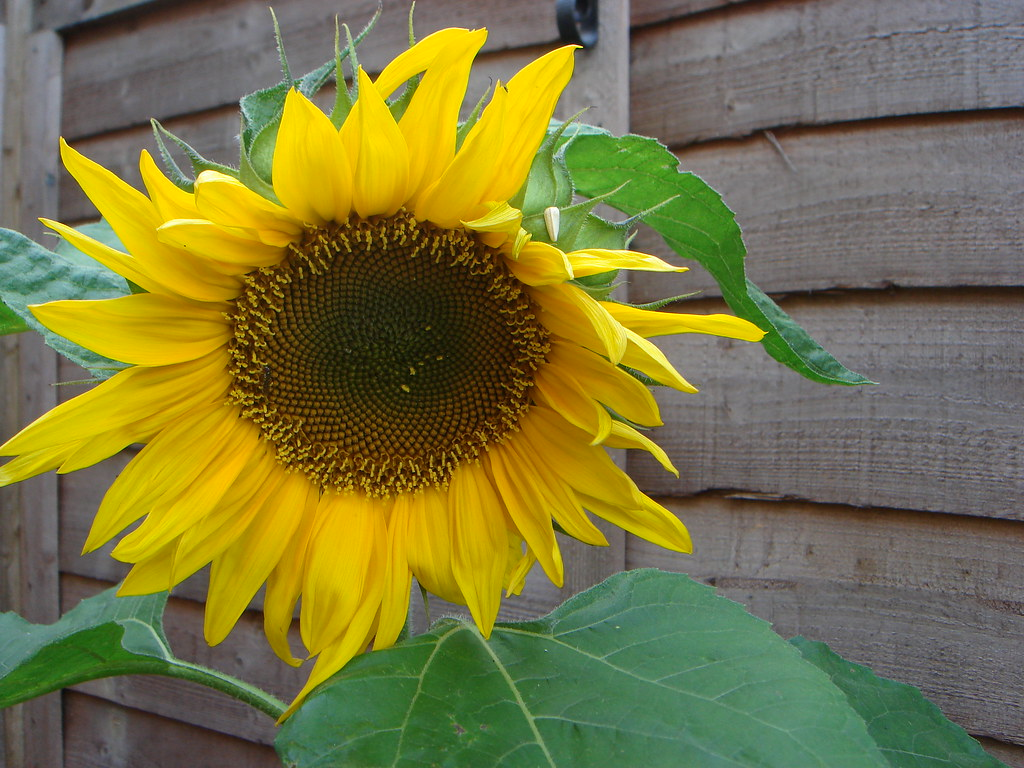
\includegraphics[width=7cm]{sunflower.jpg}
\caption{\label{sunflower}Distribution of the seeds of a sunflower (see \cite{simonbrassCCSearch2006} licenced under CC)}
\end{figure}

\section{Persian Recursion\hfill{}\textsc{Ryan}}
\label{sec:orgde8a4a3}
This section contains an example of how a simple process can lead to the
development of complex patterns when exposed to feedback and iteration.

The \emph{Persian Recursion} is a simple procedure developed by Anne Burns in the 90s
\cite{burnsPersianRecursion1997} that produces fantastic patterns when provided
with a relatively simple function.

The procedure is begins with an empty or zero square matrix with sides \(2^{n}+1,
\enspace \exists n\in \mathbb{Z}^{+}\) and some value given to the edges:

\begin{enumerate}
\item Decide on some four variable function with a finite domain and range of size \(m\), for the example shown at listing \ref{persian-recursion-python} and in figure \ref{6-rug} the function \(f(w,x,y,z)=(w+x+y+z) \mod m\) was chosen.
\item Assign this value to the centre row and centre column of the matrix
\item Repeat this for each newly enclosed subsmatrix.
\end{enumerate}

This is illustrated in figure \ref{persian-recursion-diagram}.

This can be implemented computationally by defining a function that:

\begin{itemize}
\item Takes the index of four corners enclosing a square sub-matrix of some matrix as input,
\item proceeds only if that square is some positive real value.
\item colours the centre column and row corresponding to a function of those four values
\item then calls itself on the corners of the four new sub-matrices enclosed by the
coloured row and column
\end{itemize}


\begin{figure}[htbp]
\centering
\includesvg[width=6cm]{persian}
\caption{\label{persian-recursion-diagram}Diagram of the Persian Recursion, implemented with \emph{Python} in listing \ref{persian-recursion-python}}
\end{figure}

This is demonstrated in listing \ref{persian-recursion-python} with python and produces the output shown in figures \ref{6-rug}, various interesting examples are provided in the appendix at section \ref{persian-recursion-examples}.

By mapping the values to colours, patterns emerge, this emergence of complex
patterns from simple rules is a well known and general phenomena that occurs in nature
\cite{EmergenceHowStupid2017,kivelsonDefiningEmergencePhysics2016}.

Many patterns that occur in nature can be explained by relatively simple rules
that are exposed to feedback and iteration
\cite[p. 16]{peitgenChaosFractalsNew2004}, this is a central theme of Alan
Turing's \emph{The Chemical Basis For Morphogenesis}
\cite{turingChemicalBasisMorphogenesis1952} which we hope to look in the course of
this research.

\lstset{language=ipython,label=persian-recursion-python,caption={Implementation of the persian recursion scheme in \emph{Python}},captionpos=b,numbers=none}
\begin{lstlisting}
%matplotlib inline
# m is colours
# n is number of folds
# Z is number for border
# cx is a function to transform the variables
def main(m, n, z, cx):
    import numpy as np
    import matplotlib.pyplot as plt

    # Make the Empty Matrix
    mat = np.empty([2**n+1, 2**n+1])
    main.mat = mat

    # Fill the Borders
    mat[:,0] = mat[:,-1] = mat[0,:] = mat[-1,:] = z

    # Colour the Grid
    colorgrid(0, mat.shape[0]-1, 0, mat.shape[0]-1, m)

    # Plot the Matrix
    plt.matshow(mat)

# Define Helper Functions
def colorgrid(l, r, t, b, m):
    # print(l, r, t, b)
    if (l < r -1):
        ## define the centre column and row
        mc = int((l+r)/2); mr = int((t+b)/2)

        ## Assign the colour
        main.mat[(t+1):b,mc] = cx(l, r, t, b, m)
        main.mat[mr,(l+1):r] = cx(l, r, t, b, m)

        ## Now Recall this function on the four new squares
                #l r   t   b
        colorgrid(l, mc, t, mr, m)    # NW
        colorgrid(mc, r, t, mr, m)    # NE
        colorgrid(l, mc, mr, b, m)    # SW
        colorgrid(mc, r, mr, b, m)    # SE

def cx(l, r, t, b, m):
    new_col = (main.mat[t,l] + main.mat[t,r] +  main.mat[b,l] + main.mat[b,r]) % m
    return new_col.astype(int)

main(5,6, 1, cx)
\end{lstlisting}



\begin{figure}[htbp]
\centering
\includesvg[width=6cm]{./persian-recursion-0}
\caption{\label{6-rug}Output produced by listing \ref{persian-recursion-python} with 6 folds}
\end{figure}

\section{Julia Sets\hfill{}\textsc{Ryan}}
\label{sec:org3603098}
\subsection{Introduction}
\label{sec:org2ee1c02}
Julia sets are a very interesting fractal and we hope to investigate them further in this project.
\subsection{Motivation}
\label{sec:org307af66}
Consider the iterative process \(x \rightarrow x^{2}, \enspace x \in \mathbb{R}\),
for values of \(x>1\) this process will diverge and for \(x<1\) it will converge.

Now Consider the iterative process \(z \rightarrow z^{2}, \enspace z \in \mathbb{C}\),
for values of \(\left\lvert z \right\rvert >1\) this process will diverge and for \(\left\lvert z \right\rvert <1\) it will converge.

Although this seems trivial this can be generalised.

Consider:

\begin{itemize}
\item The complex plane for \(\left\lvert z \right\rvert \leq 1\)
\item Some function \(f_{c}(z) = z^{2} + c, \quad c \leq 1 \in \mathbb{C}\) that can be used to iterate with
\end{itemize}

Every value on that plane will belong to one of the two following sets

\begin{itemize}
\item \(P_{c}\)
\begin{itemize}
\item The set of values on the plane that converge to zero (prisoners)
\item Define \(Q^{(k)}_{c}\) to be the the set of values confirmed as prisoners after \(k\) iterations of \(f_{c}\)
\begin{itemize}
\item this implies \(\lim_{k \rightarrow \infty} \left[ Q^{(k)}_{c}  \right] = P_{c}\)
\end{itemize}
\end{itemize}
\item \(E_{c}\)
\begin{itemize}
\item The set of values on the plane that tend to \(\infty\) (escapees)
\end{itemize}
\end{itemize}

In the case of \(f_{0}(z) = z^{2}\) all values \(\left\lvert z  \right \rvert \leq 1\) are bounded with \(\left\lvert z  \right \rvert = 1\) being an unstable stationary circle, but let's investigate what happens for different iterative functions like \(f_{1}(z) = z^{2} - 1\), despite how trivial this seems at first glance.

\subsection{Plotting the Sets}
\label{sec:org9ce6a1a}
Although the convergence of values may appear simple at first, we'll implement a
strategy to plot the prisoner and escape sets on the complex plane.

Because this involves iteration and \emph{Python} is a little slow, We'll denote
complex values as a vector\footnote{See figure for the obligatory \emph{XKCD} Comic} and define the operations as described in
listing \ref{complex-vec}.\footnote{This technique was adapted from Chapter 7 of \emph{Math adventures with Python} \cite{farrellMathAdventuresPython2019}}

To implement this test we'll consider a function called \texttt{escape\_test} that applies an
iteration (in this case \(f_{0}: z \rightarrow z^{2}\)) until that value diverges or converges.

While iterating with \(f_{c}\) once \(\left\lvert z \right\rvert >
\mathrm{max}\left(\left\{c, 2\}\right)\), the value must diverge because
\(\left\lvert c \rvert\right \leq 1\), so rather than record whether or not the
value converges or diverges, the \texttt{escape\_test} can instead record the number of
iterations \((k)\) until the value has crossed that boundary and this will provide
a measurement of the rate of divergence.

Then the \texttt{escape\_test} function can be mapped over a matrix, where each element
of that matrix is in turn mapped to a point on the cartesian plane, the resulting matrix
can be visualised as an image \footnote{these cascading values are much like brightness in Astronomy}, this is implemented in listing
\ref{py-circle-code} and the corresponding output shown in \ref{py-circle-plot}.

with respect to listing \ref{py-circle-code}:

\begin{itemize}
\item Observe that the \texttt{magnitude} function wasn't used:
\begin{enumerate}
\item This is because a \texttt{sqrt} is a costly operation and comparing two squares saves an operation
\end{enumerate}
\end{itemize}



\lstset{language=ipython,label=complex-vec,caption={Defining Complex Operations with vectors},captionpos=b,numbers=none}
\begin{lstlisting}
from math import sqrt
def magnitude(z):
    # return sqrt(z[0]**2 + z[1]**2)
    x = z[0]
    y = z[1]
    return sqrt(sum(map(lambda x: x**2, [x, y])))

def cAdd(a, b):
    x = a[0] + b[0]
    y = a[1] + b[1]
    return [x, y]


def cMult(u, v):
    x = u[0]*v[0]-u[1]*v[1]
    y = u[1]*v[0]+u[0]*v[1]
    return [x, y]
\end{lstlisting}

\lstset{language=ipython,label=py-circle-code,caption={Circle of Convergence of \(z\) under recursion},captionpos=b,numbers=none}
\begin{lstlisting}
%matplotlib inline
%config InlineBackend.figure_format = 'svg'
import numpy as np
def escape_test(z, num):
    ''' runs the process num amount of times and returns the count of
    divergence'''
    c = [0, 0]
    count = 0
    z1 = z  #Remember the original value that we are working with
    # Iterate num times
    while count <= num:
        dist = sum([n**2 for n in z1])
        distc = sum([n**2 for n in c])
        # check for divergence
        if dist > max(2, distc):
            #return the step it diverged on
            return count
        #iterate z
        z1 = cAdd(cMult(z1, z1), c)
        count+=1
        #if z hasn't diverged by the end
    return num



p = 0.25 #horizontal, vertical, pinch (zoom)
res = 200
h = res/2
v = res/2

pic = np.zeros([res, res])
for i in range(pic.shape[0]):
    for j in range(pic.shape[1]):
        x = (j - h)/(p*res)
        y = (i-v)/(p*res)
        z = [x, y]
        col = escape_test(z, 100)
        pic[i, j] = col

import matplotlib.pyplot as plt

plt.axis('off')
plt.imshow(pic)
# plt.show()

\end{lstlisting}


\begin{figure}[htbp]
\centering
\includesvg[width=9cm]{circle-of-convergence}
\caption{\label{py-circle-plot}Circle of Convergence for \(f_{0}: z \rightarrow z^{2}\)}
\end{figure}

This is precisely what we expected, but this is where things get interesting,
consider now the result if we apply this same procedure to \(f_{1}: z \rightarrow
z^{2} - 1\) or something arbitrary like \(f_{\frac{1}{4} + \frac{i}{2}}: z
\rightarrow z^{2} + (\frac{1}{4} + \frac{i}{2})\), the result is something
remarkebly unexpected, as shown in figures \ref{py-jl-1-plot} and \ref{py-jl-rab-plot}.


\begin{figure}[htbp]
\centering
\includesvg[width=9cm]{./julia-1}
\caption{\label{py-jl-1-plot}Circle of Convergence for \(f_{0}: z \rightarrow z^{2} - 1\)}
\end{figure}


\begin{figure}[htbp]
\centering
\includesvg[width=9cm]{./julia-rab}
\caption{\label{py-jl-rab-plot}Circle of Convergence for \(f_{\frac{1}{4} + \frac{i}{2}}: z \rightarrow z^{2} + \frac{1}{4} + \frac{i}{2}\)}
\end{figure}

To investigate this further consider the
more general function \(f_{0.8 e^{\pi i \tau}}: z \rightarrow z^{2} + 0.8 e^{\pi
i \tau}, \enspace \tau \in \mathbb{R}\), many fractals can be generated using
this set by varying the value of \(\tau\)\footnote{This approach was inspired by an animation on the \emph{Julia Set} Wikipedia article \cite{JuliaSet2020}}.

\emph{Python} is too slow for this, but the \emph{Julia} programming language, as a
compiled language, is significantly faster and has the benefit of treating
complex numbers as first class citizens, these images can be generated in
\emph{Julia} in a similar fashion as before, with the specifics shown in listing
\ref{julia-gen-fracs}. The \texttt{GR} package appears to be the best plotting library
performance wise and so was used to save corresponding images to disc, this is
demonstrated in listing \ref{GR-save} where 1200 pictures at a 2.25 MP resolution were produced. \footnote{On my system this took about 30 minutes.}

A subset of these images can be combined using \emph{ImageMagick} and \texttt{bash} to
create a collage, \emph{ImageMagick} can also be used to produce an animation but it often
fails and a superior approach is to use \texttt{ffmpeg}, this is demonstrated in
listing \ref{bash-frac-join}, the collage is shown in figure \ref{montage-frac} and a corresponding
animation is \href{https://dl.dropboxusercontent.com/s/rbu25urfg8sbwfu/out.gif?dl=0}{available online}\footnote{\href{https://dl.dropboxusercontent.com/s/rbu25urfg8sbwfu/out.gif?dl=0}{https://dl.dropboxusercontent.com/s/rbu25urfg8sbwfu/out.gif?dl=0}}].

\lstset{language=julia,label=julia-gen-fracs,caption={Produce a series of fractals using julia},captionpos=b,numbers=none}
\begin{lstlisting}
# * Define the Julia Set
"""
Determine whether or not a value will converge under iteration
"""
function juliaSet(z, num, my_func)
    count = 1
    # Remember the value of z
    z1 = z
    # Iterate num times
    while count ≤ num
        # check for divergence
        if abs(z1)>2
            return Int(count)
        end
        #iterate z
        z1 = my_func(z1) # + z
        count=count+1
    end
        #if z hasn't diverged by the end
    return Int(num)
end

# * Make a Picture
"""
Loop over a matrix and apply apply the julia-set function to
the corresponding complex value
"""
function make_picture(width, height, my_func)
    pic_mat = zeros(width, height)
    zoom = 0.3
    for i in 1:size(pic_mat)[1]
        for j in 1:size(pic_mat)[2]
            x = (j-width/2)/(width*zoom)
            y = (i-height/2)/(height*zoom)
            pic_mat[i,j] = juliaSet(x+y*im, 256, my_func)
        end
    end
    return pic_mat
end

\end{lstlisting}

\lstset{language=julia,label=GR-save,caption={Generate and save the images with GR},captionpos=b,numbers=none}
\begin{lstlisting}
# * Use GR to Save a Bunch of Images
  ## GR is faster than PyPlot
using GR
function save_images(count, res)
    try
        mkdir("/tmp/gifs")
    catch
    end
    j = 1
    for i in (1:count)/(40*2*π)
        j = j + 1
        GR.imshow(make_picture(res, res, z -> z^2 + 0.8*exp(i*im*9/2))) # PyPlot uses interpolation = "None"
        name = string("/tmp/gifs/j", lpad(j, 5, "0"), ".png")
        GR.savefig(name)
    end
end

save_images(1200, 1500) # Number  and Res
\end{lstlisting}

\lstset{language=bash,label=bash-frac-join,caption={Using \texttt{bash}, \texttt{ffmpeg} and \emph{ImageMagick} to combine the images and produce an animation.},captionpos=b,numbers=none}
\begin{lstlisting}
# Use montage multiple times to get recursion for fun
montage (ls *png | sed -n '1p;0~600p') 0a.png
montage (ls *png | sed -n '1p;0~100p') a.png
montage (ls *png | sed -n '1p;0~50p') -geometry 1000x1000  a.png

# Use ImageMagick to Produce a gif (unreliable)
convert -delay 10 *.png 0.gif

# Use FFMpeg to produce a Gif instead
ffmpeg                    \
    -framerate 60         \
    -pattern_type glob    \
    -i '*.png'            \
    -r 15                 \
    out.mov


\end{lstlisting}

\begin{figure}[htbp]
\centering
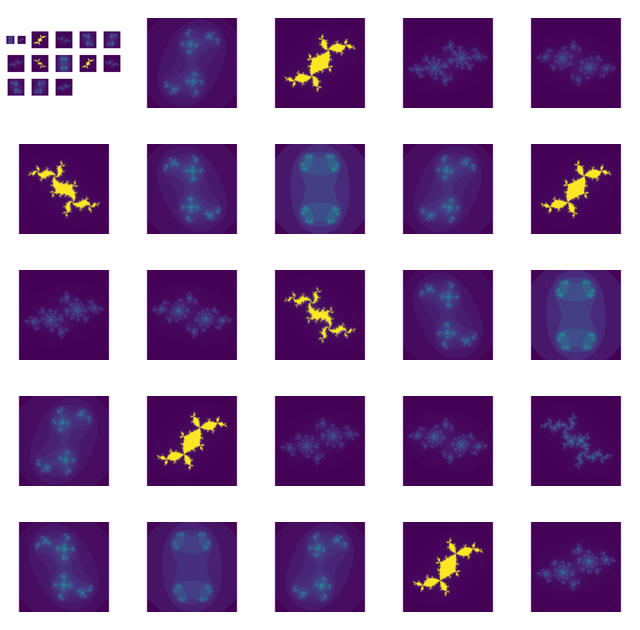
\includegraphics[width=.9\linewidth]{/home/ryan/Dropbox/Studies/2020Spring/QuantProject/Current/Python-Quant/Outline/_20200826_005334a.png}
\caption{\label{montage-frac}Various fracals corresponding to \(f_{0.8 e^{\pi i \tau}}\)}
\end{figure}

\section{MandelBrot\hfill{}\textsc{Ryan}}
\label{sec:org11ca13f}
Investigating these fractals, a natural question might be whether or not any
given \(c\) value will produce a fractal that is an open disc or a closed disc.

So pick a value \(\left\lvert \gamma \right \rvert < 1\) in the complex plane and
use it to produce the julia set \(f_{\gamma}\), if the corresponding prisoner set
\(P\) is closed we this value is defined as belonging to the \emph{Mandelbrot} set.

It can be shown (and I intend to show it generally), that this set is equivalent to re-implementing the previous strategy such that \(z \rightarrow z^{2} + z_{0}\) where \(z_{0}\) is unchanging or more clearly as a seqeuence:

\begin{align}
z_{n+1} &= z^{2}_n + c \label{eq:mb-sequence} \\
z_{0}   &= c
\end{align}

This strategy is implemented in listing and produces the output shown in figure \ref{mandelbrot-py-pic}.

\lstset{language=ipython,label=py-mandelbrot-code,caption={All values of \(c\) that lead to a closed \emph{Julia-set}},captionpos=b,numbers=none}
\begin{lstlisting}
%matplotlib inline
%config InlineBackend.figure_format = 'svg'
def mandelbrot(z, num):
    ''' runs the process num amount of times and returns the count of
    divergence'''
    count = 0
    # Define z1 as z
    z1 = z
    # Iterate num times
    while count <= num:
        # check for divergence
        if magnitude(z1) > 2.0:
            #return the step it diverged on
            return count
        #iterate z
        z1 = cAdd(cMult(z1, z1),z)
        count+=1
        #if z hasn't diverged by the end
    return num

import numpy as np


p = 0.25 # horizontal, vertical, pinch (zoom)
res = 200
h = res/2
v = res/2

pic = np.zeros([res, res])
for i in range(pic.shape[0]):
    for j in range(pic.shape[1]):
        x = (j - h)/(p*res)
        y = (i-v)/(p*res)
        z = [x, y]
        col = mandelbrot(z, 100)
        pic[i, j] = col

import matplotlib.pyplot as plt
plt.imshow(pic)
# plt.show()
\end{lstlisting}

\begin{figure}[htbp]
\centering
\includesvg[width=8cm]{./mandelbrot-py}
\caption{\label{mandelbrot-py-pic}Mandelbrot Set produced in \emph{Python} as shown in listing \ref{py-mandelbrot-code}}
\end{figure}

This output although remarkable is however fairly undetailed, by using \emph{Julia} a much
larger image can be produced, in \emph{Julia} producing a 4 GB, 400 MP image can be done in little time
(about 10 minutes on my system), this is demonstrated in listing 
and the corresponding FITS image is \href{https://www.dropbox.com/s/jd5qf1pi2h68f2c/mandelbrot-400mpx.fits?dl=0}{available-online.}\footnote{\href{https://www.dropbox.com/s/jd5qf1pi2h68f2c/mandelbrot-400mpx.fits?dl=0}{https://www.dropbox.com/s/jd5qf1pi2h68f2c/mandelbrot-400mpx.fits?dl=0}}

\lstset{language=julia,label,caption= ,captionpos=b,numbers=none}
\begin{lstlisting}
function mandelbrot(z, num, my_func)
    count = 1
    # Define z1 as z
    z1 = z
    # Iterate num times
    while count ≤ num
        # check for divergence
        if abs(z1)>2
            return Int(count)
        end
        #iterate z
        z1 = my_func(z1) + z
        count=count+1
    end
        #if z hasn't diverged by the end
    return Int(num)
end

function make_picture(width, height, my_func)
    pic_mat = zeros(width, height)
    for i in 1:size(pic_mat)[1]
        for j in 1:size(pic_mat)[2]
            x = j/width
            y = i/height
            pic_mat[i,j] = mandelbrot(x+y*im, 99, my_func)
        end
    end
    return pic_mat
end


using FITSIO
function save_picture(filename, matrix)
    f = FITS(filename, "w");
    # data = reshape(1:100, 5, 20)
    # data = pic_mat
    write(f, matrix)  # Write a new image extension with the data

    data = Dict("col1"=>[1., 2., 3.], "col2"=>[1, 2, 3]);
    write(f, data)  # write a new binary table to a new extension

    close(f)
end

# * Save Picture
#------------------------------------------------------------
my_pic = make_picture(20000, 20000, z -> z^2) 2000^2 is 4 GB
save_picture("/tmp/a.fits", my_pic)

\end{lstlisting}

\begin{figure}[htbp]
\centering
\includegraphics[width=10cm]{_20200828_233844screenshot.png}
\caption{\label{mandelbrot-screen}Screenshot of Mandelbrot FITS image produced by listing }
\end{figure}
\section{Relevant Sources}
\label{sec:org3d8f7f0}
To guide research for our topic \emph{Chaos and Fractals} by Pietgen, Jurgens and Saupe \cite{peitgenChaosFractalsNew2004} will act as a map of the topic broadly, other than the sources referenced already, we anticipate referring to the following textbooks that we access to throughout the project:

\begin{itemize}
\item \emph{Integration of Fuzzy Logic and Chaos Theory}      \cite{liIntegrationFuzzyLogic2006}
\item \emph{Advances in Chaos Theory and Intelligent Control} \cite{azarAdvancesChaosTheory2016}
\item \emph{NonLinear Dynamics and Chaos}                     \cite{strogatzNonlinearDynamicsChaos2015}
\item \emph{The NonLinear Universe}                           \cite{scottNonlinearUniverseChaos2007}
\item \emph{Chaos and Fractals}                               \cite{peitgenChaosFractalsNew2004}
\item \emph{Turbulent Mirror}                                 \cite{briggsTurbulentMirrorIllustrated1989}
\item \emph{Fractal Geometry}                                 \cite{falconerFractalGeometryMathematical2003b}
\item \emph{Math Adventures with Python}                      \cite{farrellMathAdventuresPython2019}
\item \emph{The Topology of Chaos}                            \cite{gilmoreTopologyChaosAlice2002}
\item \emph{Chaotic Dynamics}                                 \cite{telChaoticDynamicsIntroduction2006}
\end{itemize}

Ron Knott's website appears also to have a lot of material related to patterns, the \emph{Fibonacci Sequence} and the \emph{Golden Ratio}, we intend to have a good look through that material as well. \cite{ronknottFibonacciNumbersGolden2016}

\section{Appendix}
\label{sec:org04bbdc8}

\lstset{language=Python,label=py-env,caption={Preamble for \emph{Python} Environment},captionpos=b,numbers=none}
\begin{lstlisting}
  from __future__ import division
  from sympy import *
  x, y, z, t = symbols('x y z t')
  k, m, n = symbols('k m n', integer=True)
  f, g, h = symbols('f g h', cls=Function)
  init_printing()
  init_printing(use_latex='mathjax', latex_mode='equation')


  import pyperclip
  def lx(expr):
      pyperclip.copy(latex(expr))
      print(expr)

  import numpy as np
  import matplotlib as plt

  import time

  def timeit(k):
      start = time.time()
      k
      print(str(round(time.time() - start, 9)) + "seconds")
\end{lstlisting}

\subsection{Persian Recursian Examples}
\label{persian-recursion-examples}
\lstset{language=ipython,label=8-fold-code,caption={Enhance listing \ref{persian-recursion-python} to create 9 folds},captionpos=b,numbers=none}
\begin{lstlisting}
%config InlineBackend.figure_format = 'svg'
main(5, 9, 1, cx)
\end{lstlisting}
\begin{center}
\includesvg[width=.9\linewidth]{./persian-recursion-large}
\end{center}


\lstset{language=ipython,label=new-func-code,caption={Modify the Function to use \(f(w,x,y,z) = (w + x + y + z - 7) \mod 8\)},captionpos=b,numbers=none}
\begin{lstlisting}
%config InlineBackend.figure_format = 'svg'
def cx(l, r, t, b, m):
    new_col = (main.mat[t,l] + main.mat[t,r] +  main.mat[b,l] + main.mat[b,r]-7) % m
    return new_col.astype(int)
main(8, 8, 1, cx)
\end{lstlisting}

\begin{figure}[htbp]
\centering
\includesvg[width=9cm]{./persian-recursion-new-func}
\caption{\label{new-func-plot}Output produced by listing \ref{new-func-code} using \(f(w,x,y,z) = (w + x + y + z - 7) \mod 8\)}
\end{figure}


\lstset{language=ipython,label=new-func2-code,caption={Modify the function to use \(f(w,x,y,z) = (w + 8x + 8y + 8z) \mod 8 + 1\)},captionpos=b,numbers=none}
\begin{lstlisting}
%config InlineBackend.figure_format = 'svg'
import numpy as np
def cx(l, r, t, b, m):
    new_col = (main.mat[t,l] + main.mat[t,r]*m +  main.mat[b,l]*(m) + main.mat[b,r]*(m))**1 % m + 1
    return new_col.astype(int)
main(8, 8, 1, cx)
\end{lstlisting}


\begin{figure}[htbp]
\centering
\includesvg[width=9cm]{./persian-recursion-new-func2}
\caption{\label{new-func2-plot}Output produced by listing \ref{new-func2-code} using \(f(w,x,y,z) = (w + 8x + 8y + 8z) \mod 8 + 1\)}
\end{figure}
\subsection{Figures}
\label{sec:org6a3e73c}

\begin{figure}[htbp]
\centering
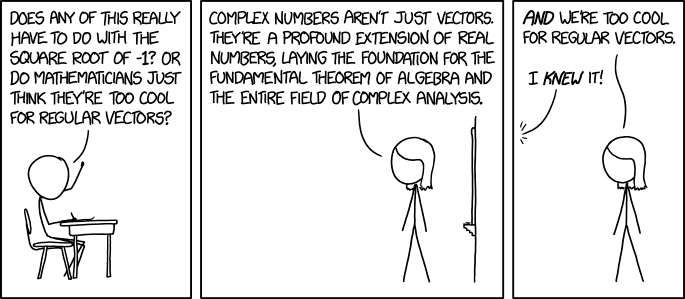
\includegraphics[width=.9\linewidth]{complex_numbers.png}
\caption{\label{xkcd-complex-numbers}XKCD 2028: Complex Numbers}
\end{figure}
\subsection{Why Julia}
\label{why-julia}
The reason we resolved to make time to investigate \emph{Julia} is because we see it as a very important tool for mathematics in the future, in particular because:

\begin{itemize}
\item It is a new modern language, designed primarily with mathematics in mind
\begin{itemize}
\item First class support for UTF8 symbols
\item Full Support to call \emph{\textbf{R}} and \emph{Python}.
\end{itemize}
\item Performance wise it is best in class and only rivalled by compiled languages such as \emph{Fortran} \emph{Rust} and \textbf{\emph{C}}
\begin{itemize}
\item \emph{Just in Time Compiling} allows for a very useable \emph{REPL} making Julia
significantly more appealing than compiled languages
\item The syntax of Julia is very similar to \emph{Python} and \emph{\textbf{R}}
\end{itemize}
\item The \texttt{DifferentialEquations.jl} library is one of the best performing libraries available.
\end{itemize}

\paragraph{Other Packages}
\label{other-tools}
Other packages that are on our radar for want of investigation are listed below, in practice it is unlikely that time will permit us to investigate many packages or libraries

\begin{itemize}
\item Programming Languages and CAS
\begin{itemize}
\item Julia
\begin{itemize}
\item SymEngine.jl
\item Symata.jl
\item SymPy.jl
\end{itemize}
\item Maxima
\begin{itemize}
\item Being the oldest there is probably a lot too learn
\end{itemize}
\item Julia
\item Reduce
\item Xcas/Gias
\item Python
\begin{itemize}
\item Numpy
\item Sympy
\end{itemize}
\end{itemize}
\item Visualisation
\begin{itemize}
\item Makie
\item Plotly
\item GNUPlot
\end{itemize}
\end{itemize}
\end{document}
